% Transition Diagrams for Exercise 3.6.1
% Author		: Finn Rayment
% Date created	: 17-03-2019
%

\documentclass{article}

\usepackage{tikz}
\usetikzlibrary{automata, positioning, arrows}

\begin{document}

\begin{figure}[ht]
\centering
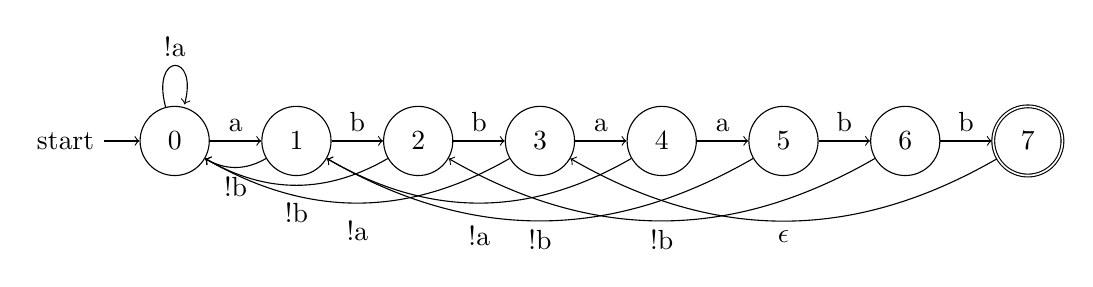
\begin{tikzpicture}[bend angle=30]
	\node[state, initial] (q1) {0};
	\node[state, right of=q1, right=0.1cm] (q2) {1};
	\node[state, right of=q2, right=0.1cm] (q3) {2};
	\node[state, right of=q3, right=0.1cm] (q4) {3};
	\node[state, right of=q4, right=0.1cm] (q5) {4};
	\node[state, right of=q5, right=0.1cm] (q6) {5};
	\node[state, right of=q6, right=0.1cm] (q7) {6};
	\node[state, right of=q7, right=0.1cm, accepting] (q8) {7};

	\draw [->]
		(q1) edge[above] node{a} (q2)
		(q2) edge[above] node{b} (q3)
		(q3) edge[above] node{b} (q4)
		(q4) edge[above] node{a} (q5)
		(q5) edge[above] node{a} (q6)
		(q6) edge[above] node{b} (q7)
		(q7) edge[above] node{b} (q8)

		(q1) edge[loop above] node{!a} (q1)

		(q2) edge[bend left, below] node{!b} (q1)
		(q3) edge[bend left, below] node[yshift=-3]{!b} (q1)
		(q4) edge[bend left, below] node[yshift=-3]{!a} (q1)
		(q5) edge[bend left, below] node[yshift=-5]{!a} (q2)
		(q6) edge[bend left, below] node{!b} (q2)
		(q7) edge[bend left, below] node{!b} (q3)
		(q8) edge[bend left, below] node{$\epsilon$} (q4)
		;
\end{tikzpicture}
\caption{DFA that recognises .*$b_{1}b_{2} \ldots b_{n}$ where the dot stands for "any character".}
\label{fig:a}
\end{figure}

\end{document}
